
\documentclass{article}
\usepackage[utf8]{inputenc}
\usepackage{amsmath}
\usepackage{amsfonts}
\usepackage{amssymb}
\usepackage{graphicx}
\usepackage{booktabs}
\usepackage{caption}   % Paquete para personalizar leyendas de figuras
\usepackage{float}     % Paquete para la opción `H` en figuras
\usepackage{subcaption} % Añadir al preámbulo
% Configuración del título

    
    \title{Informe de Análisis Exploratorio de \texttt{mtcars}}
    \author{
      Melani Forsythe Matos \\
      Daniela Guerrero Álvarez \\
      Rubén Martínez Rojas
    }
    \date{} % Sin fecha para que no aparezca
    
\begin{document}

\maketitle

\newpage % Inserta una nueva página aquí


El conjunto de datos \texttt{mtcars} en R es un conjunto clásico que contiene datos sobre automóviles, y tiene 32 observaciones (filas) de 11 variables (columnas). A continuación, describo cada una de las variables, su significado, el tipo de escala, y si son discretas o continuas:

\begin{enumerate}
    \item \textbf{mpg (Miles per Gallon)}

          \begin{itemize}
              \item \textbf{Descripción:} Consumo de combustible del automóvil en millas por galón.
              \item \textbf{Escala:} Cuantitativa Continua.
              \item \textbf{Significado:} Representa la eficiencia del combustible del automóvil, es decir, cuántas millas puede recorrer el automóvil por cada galón de gasolina.
          \end{itemize}

          \begin{figure}[H]
              \centering
              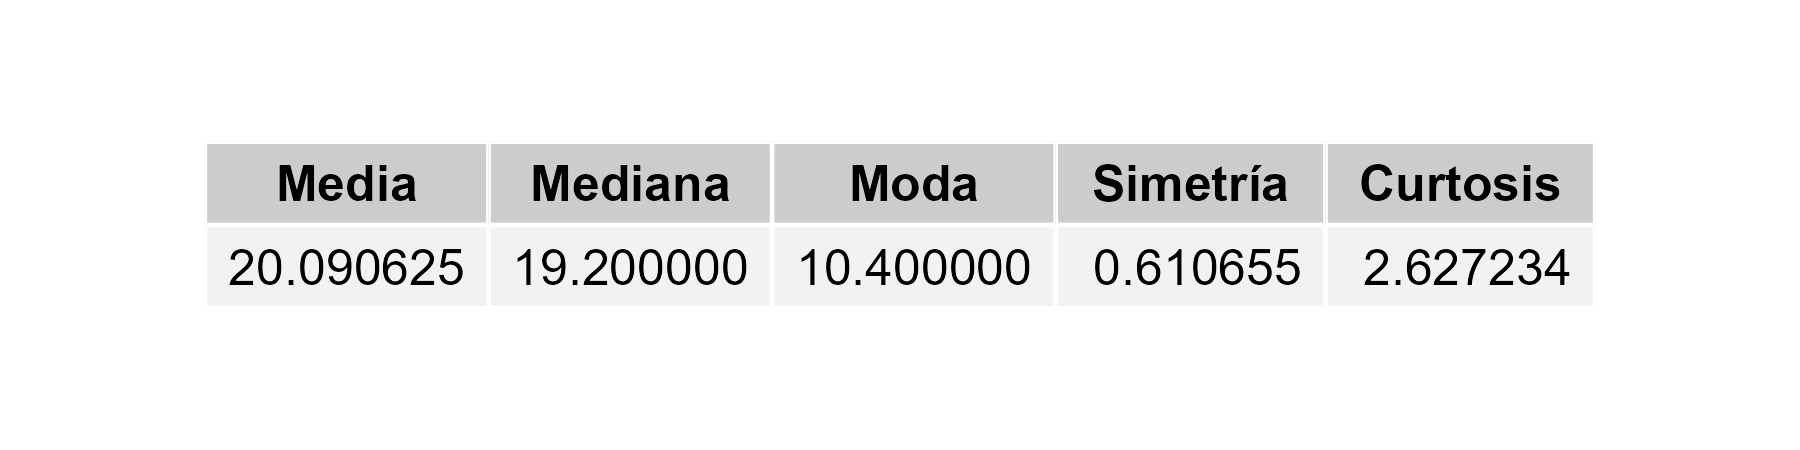
\includegraphics[width=0.8\textwidth]{MTC/mpg_central.png}
              \caption{Medidas de tendencia central para la variable \texttt{mpg}.}
              \label{fig:mpg_central}
          \end{figure}

          \begin{figure}[H]
              \centering
              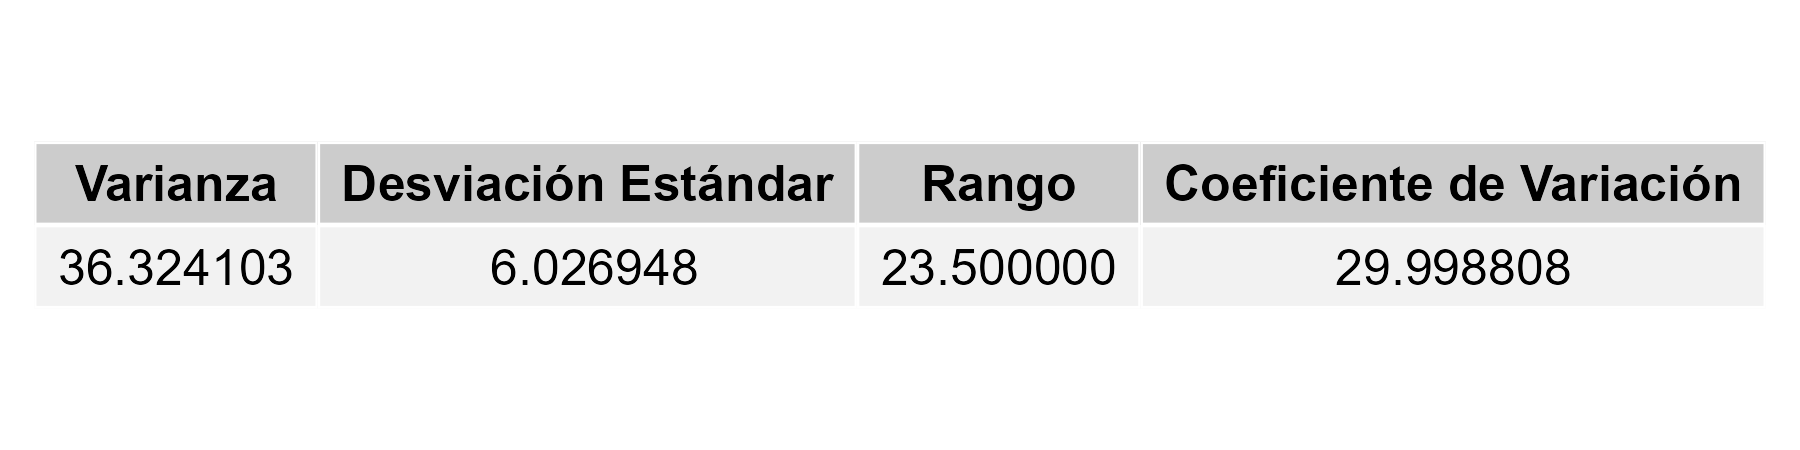
\includegraphics[width=0.8\textwidth]{MTC/mpg_dispersion.png}
              \caption{Medidas de dispersión para la variable \texttt{mpg}.}
              \label{fig:mpg_dispersion}
          \end{figure}

    \item \textbf{cyl (Cylinders)}

          \begin{itemize}
              \item \textbf{Descripción:} Número de cilindros en el motor del automóvil.
              \item \textbf{Escala:} Cuantitativa Discreta.
              \item \textbf{Significado:} Indica cuántos cilindros tiene el motor. Generalmente, los valores comunes son 4, 6 u 8 cilindros.
          \end{itemize}

          \begin{figure}[H]
              \centering
              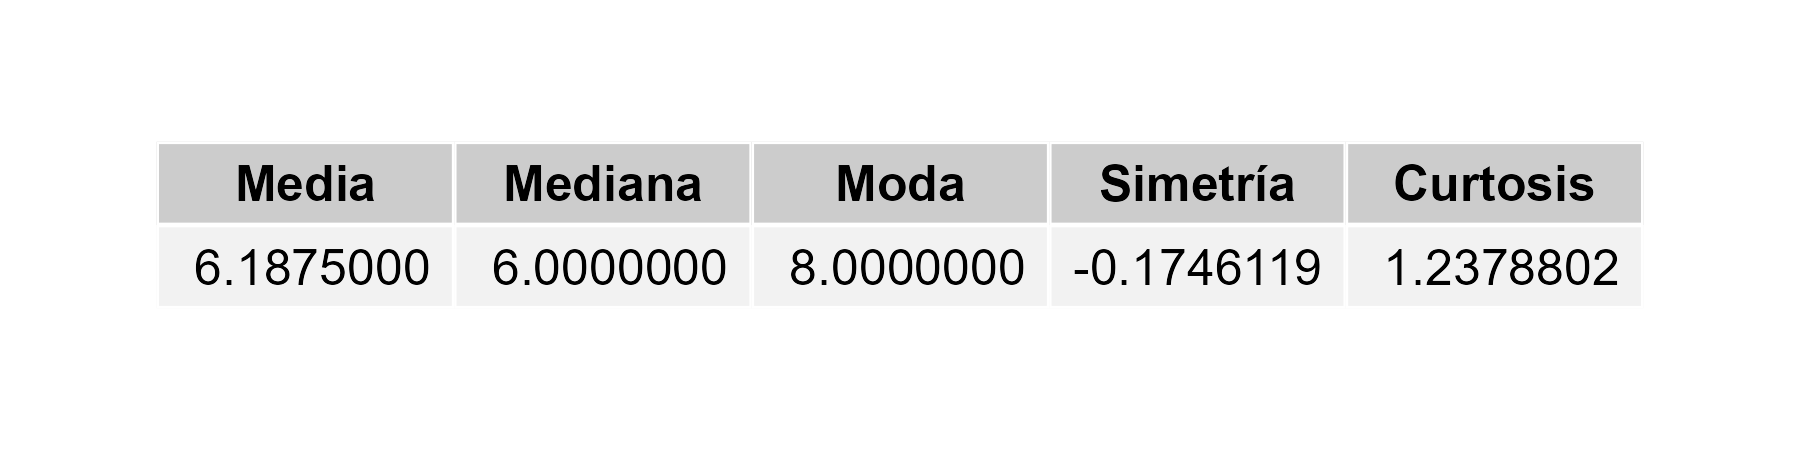
\includegraphics[width=0.8\textwidth]{MTC/cyl_central.png}
              \caption{Medidas de tendencia central para la variable \texttt{cyl}.}
              \label{fig:cyl_central}
          \end{figure}

          \begin{figure}[H]
              \centering
              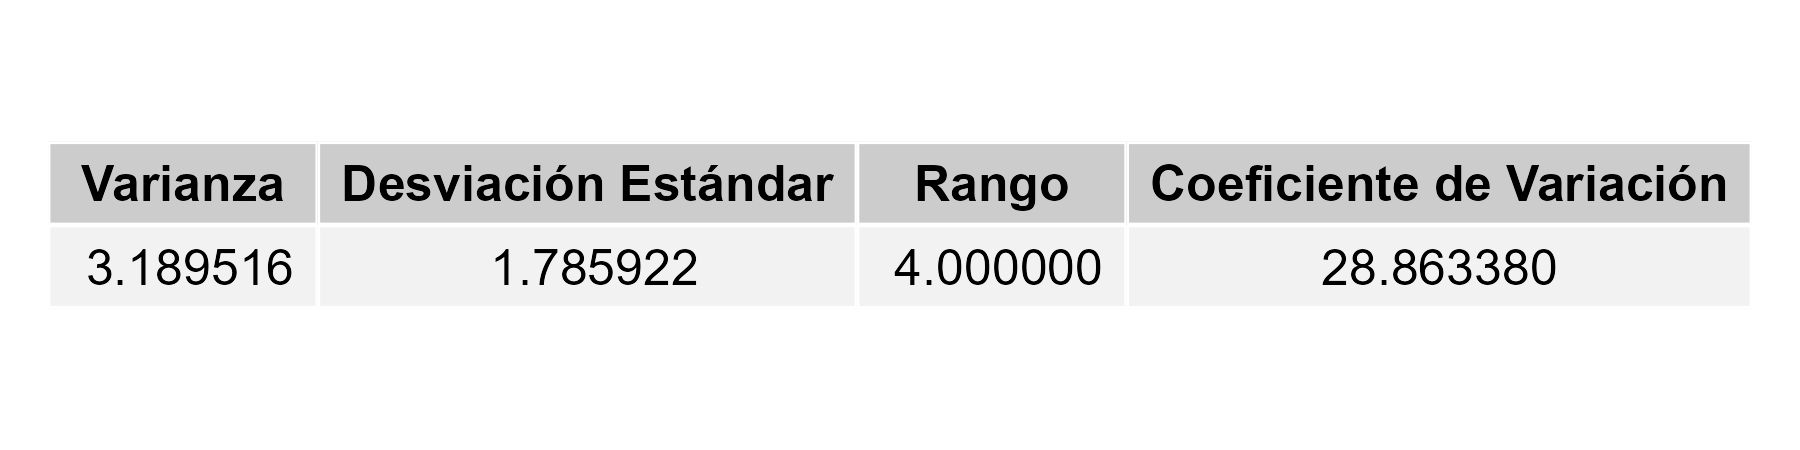
\includegraphics[width=0.8\textwidth]{MTC/cyl_dispersion.png}
              \caption{Medidas de dispersión para la variable \texttt{cyl}.}
              \label{fig:cyl_dispersion}
          \end{figure}

    \item \textbf{disp (Displacement)}

          \begin{itemize}
              \item \textbf{Descripción:} Desplazamiento del motor en pulgadas cúbicas.
              \item \textbf{Escala:} Cuantitativa Continua.
              \item \textbf{Significado:} Es el volumen total desplazado por todos los pistones dentro del motor en una sola revolución. Es una medida del tamaño del motor.
          \end{itemize}

          \begin{figure}[H]
              \centering
              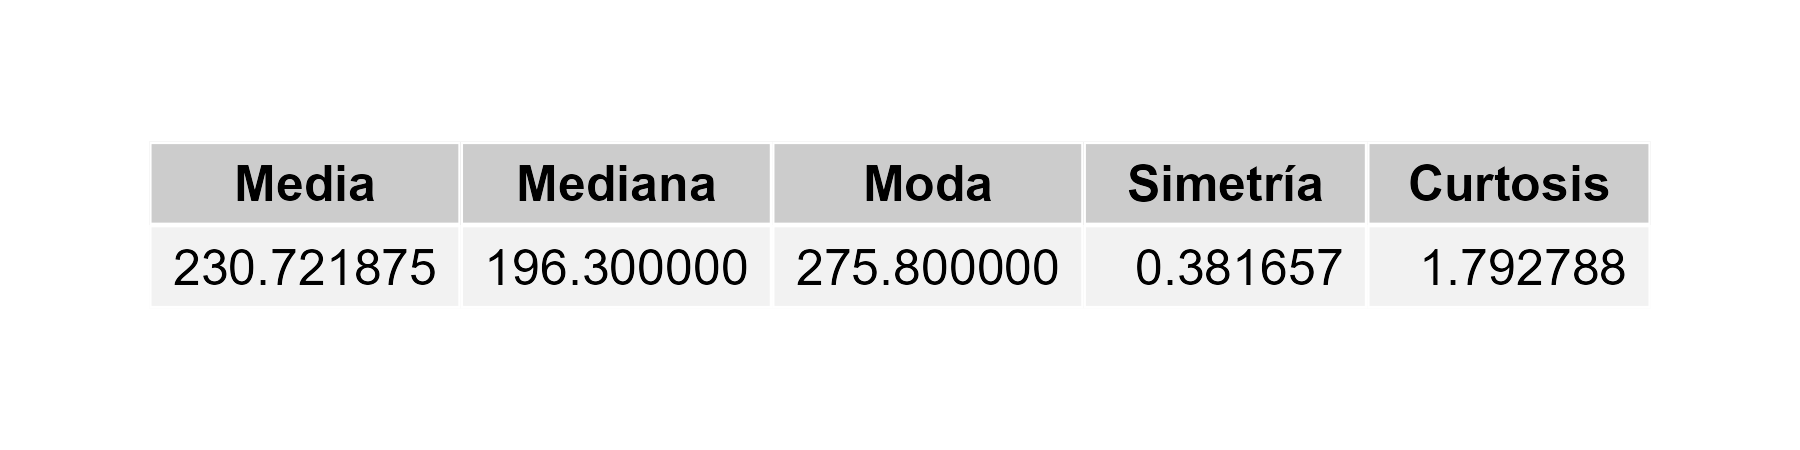
\includegraphics[width=0.8\textwidth]{MTC/disp_central.png}
              \caption{Medidas de tendencia central para la variable \texttt{disp}.}
              \label{fig:disp_central}
          \end{figure}

          \begin{figure}[H]
              \centering
              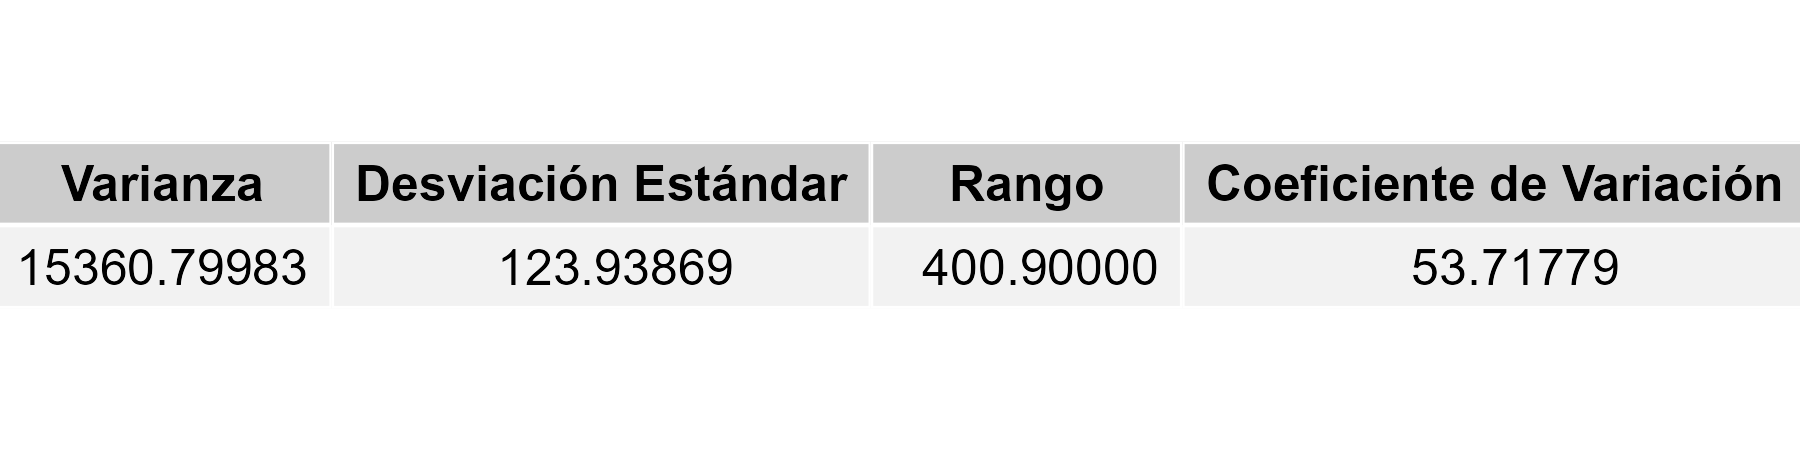
\includegraphics[width=0.8\textwidth]{MTC/disp_dispersion.png}
              \caption{Medidas de dispersión para la variable \texttt{disp}.}
              \label{fig:disp_dispersion}
          \end{figure}

    \item \textbf{hp (Horsepower)}

          \begin{itemize}
              \item \textbf{Descripción:} Potencia del motor en caballos de fuerza.
              \item \textbf{Escala:} Es una variable Cuantitativa que puede tener valores Continuos, pero en este caso solo guarda valores Discretos, por tanto la trataremos como Cuantitativa Discreta.
              \item \textbf{Significado:} Mide la potencia del motor, es decir, la capacidad del motor para realizar trabajo en una unidad de tiempo.
          \end{itemize}

          \begin{figure}[H]
              \centering
              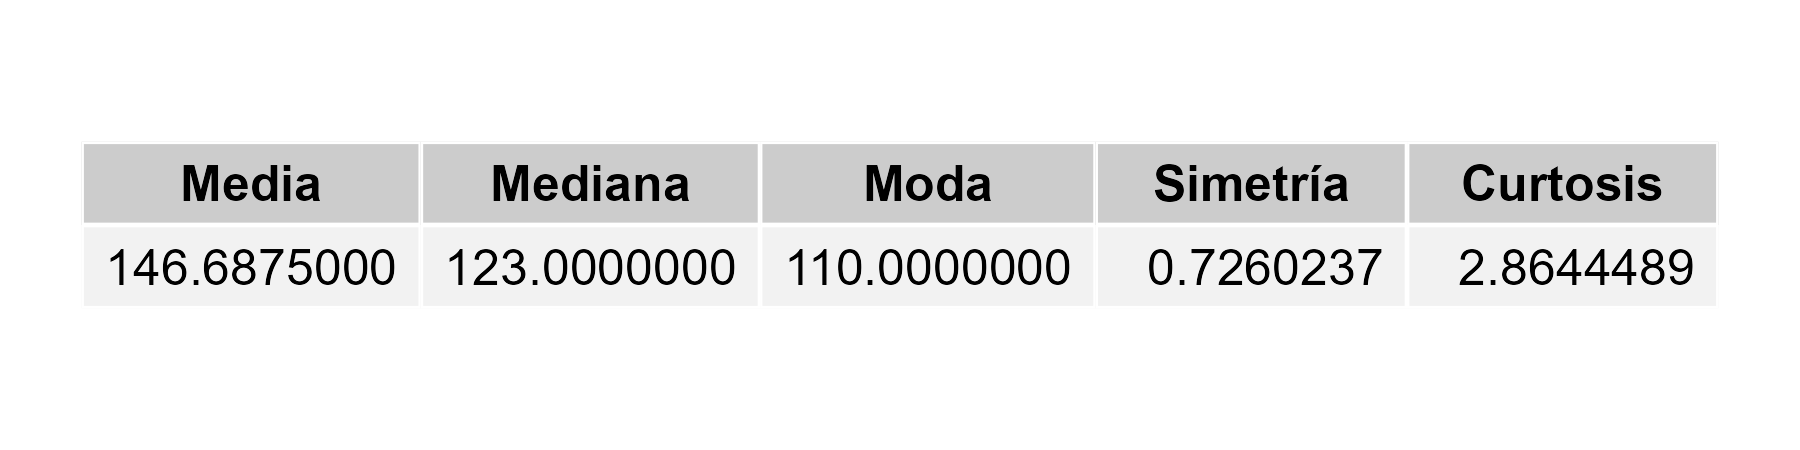
\includegraphics[width=0.8\textwidth]{MTC/hp_central.png}
              \caption{Medidas de tendencia central para la variable \texttt{hp}.}
              \label{fig:hp_central}
          \end{figure}

          \begin{figure}[H]
              \centering
              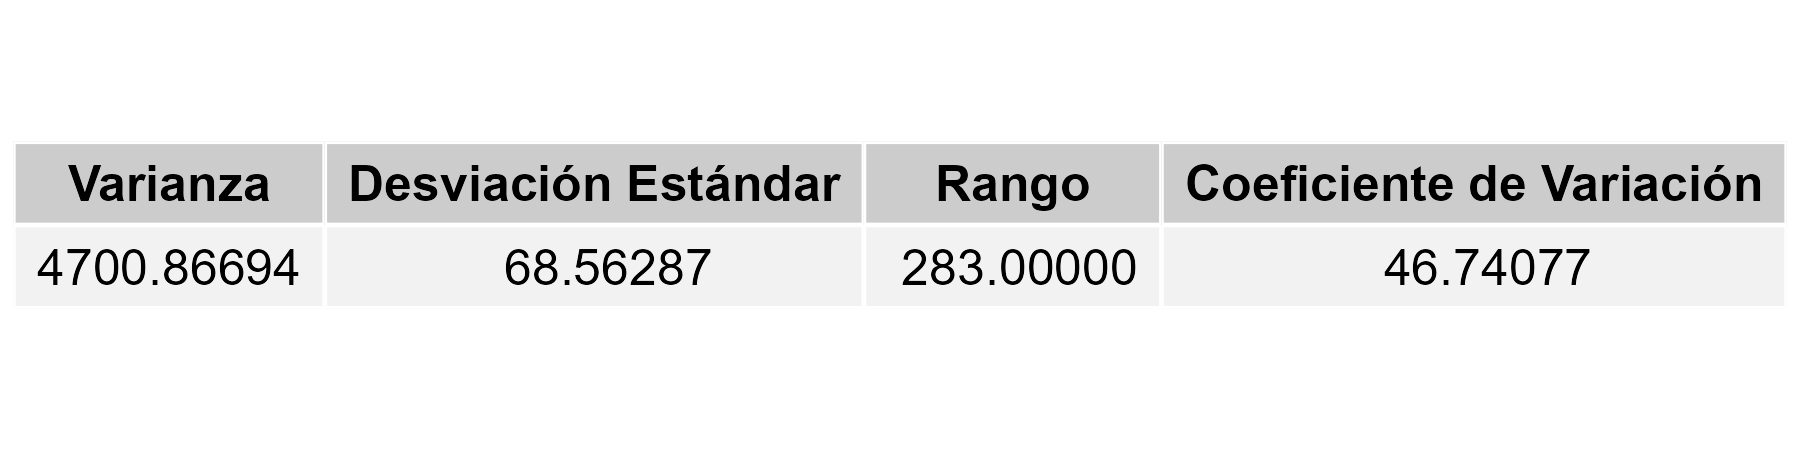
\includegraphics[width=0.8\textwidth]{MTC/hp_dispersion.png}
              \caption{Medidas de dispersión para la variable \texttt{hp}.}
              \label{fig:hp_dispersion}
          \end{figure}

    \item \textbf{drat (Rear Axle Ratio)}

          \begin{itemize}
              \item \textbf{Descripción:} Relación de transmisión del eje trasero.
              \item \textbf{Escala:} Cuantitativa Continua.
              \item \textbf{Significado:} Es la relación entre las revoluciones del eje de transmisión y las revoluciones del eje trasero. Afecta el rendimiento y la velocidad del vehículo.
          \end{itemize}

          \begin{figure}[H]
              \centering
              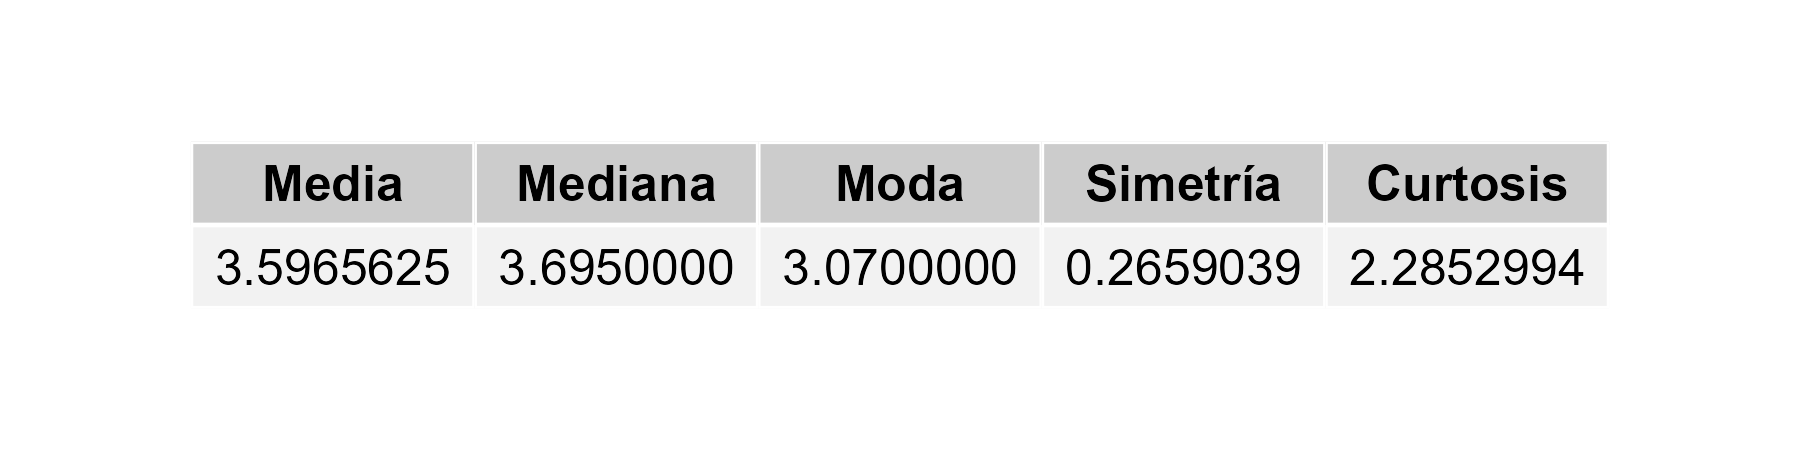
\includegraphics[width=0.8\textwidth]{MTC/drat_central.png}
              \caption{Medidas de tendencia central para la variable \texttt{drat}.}
              \label{fig:drat_central}
          \end{figure}

          \begin{figure}[H]
              \centering
              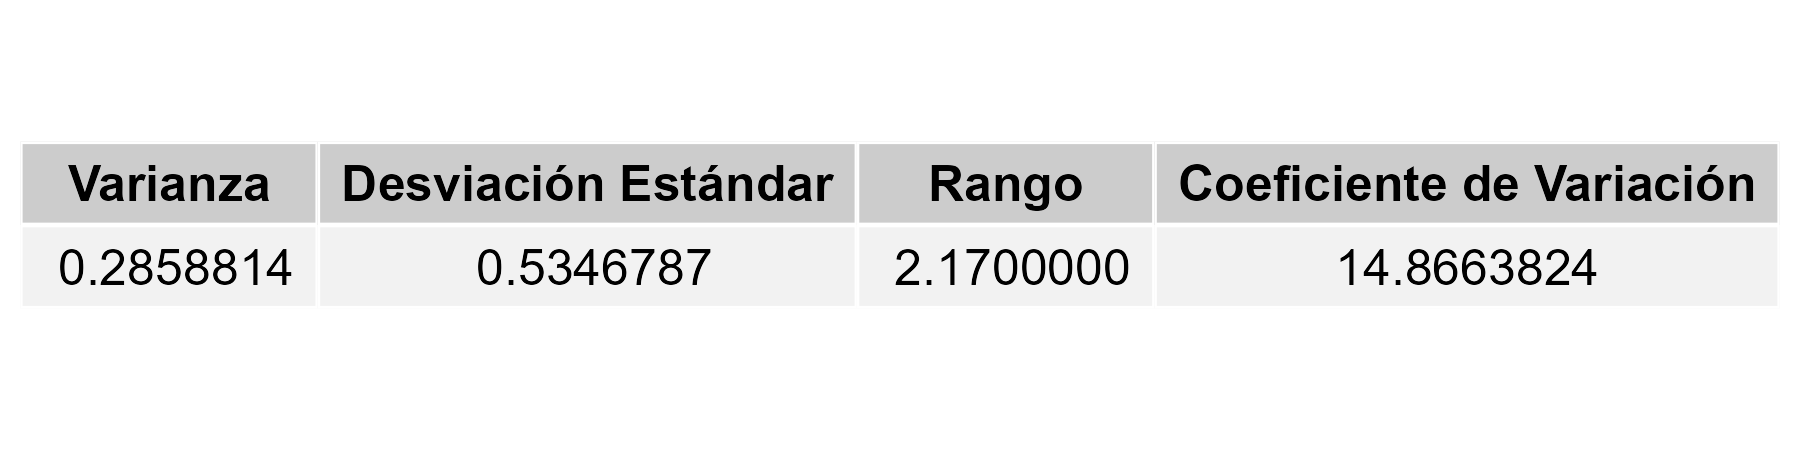
\includegraphics[width=0.8\textwidth]{MTC/drat_dispersion.png}
              \caption{Medidas de dispersión para la variable \texttt{drat}.}
              \label{fig:drat_dispersion}
          \end{figure}

    \item \textbf{wt (Weight)}

          \begin{itemize}
              \item \textbf{Descripción:} Peso del automóvil en miles de libras.
              \item \textbf{Escala:} Cuantitativa Continua.
              \item \textbf{Significado:} El peso del automóvil influye en su eficiencia, aceleración y manejo.
          \end{itemize}

          \begin{figure}[H]
              \centering
              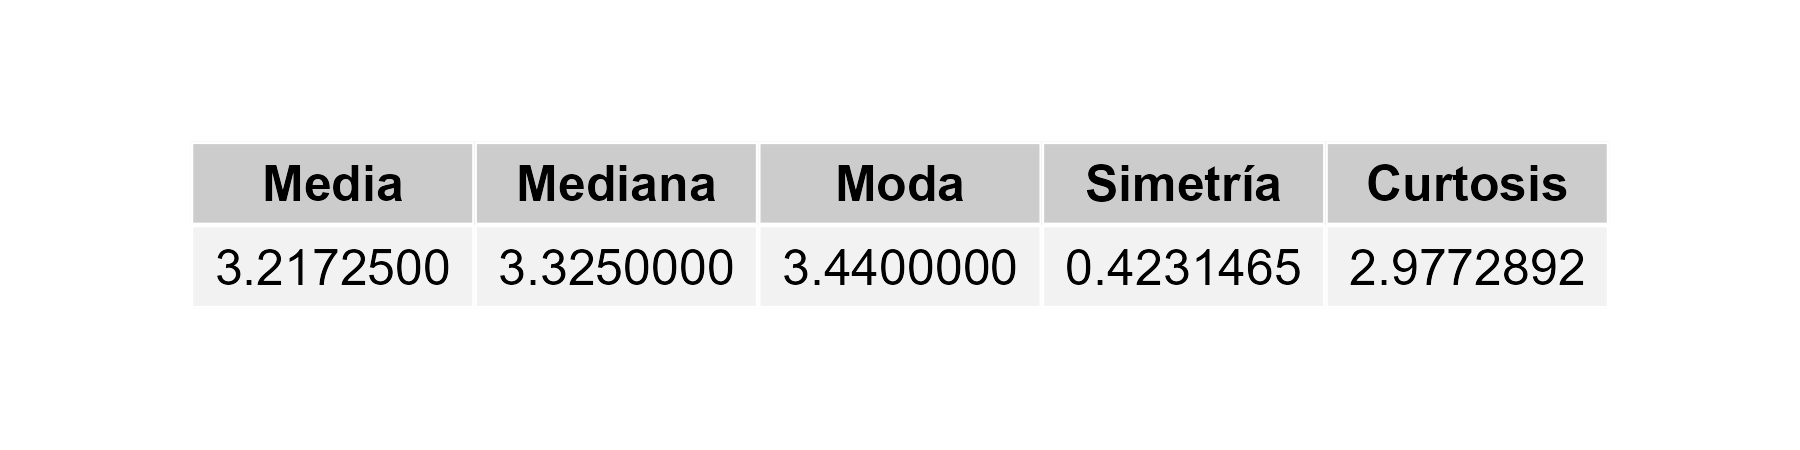
\includegraphics[width=0.8\textwidth]{MTC/wt_central.png}
              \caption{Medidas de tendencia central para la variable \texttt{wt}.}
              \label{fig:wt_central}
          \end{figure}

          \begin{figure}[H]
              \centering
              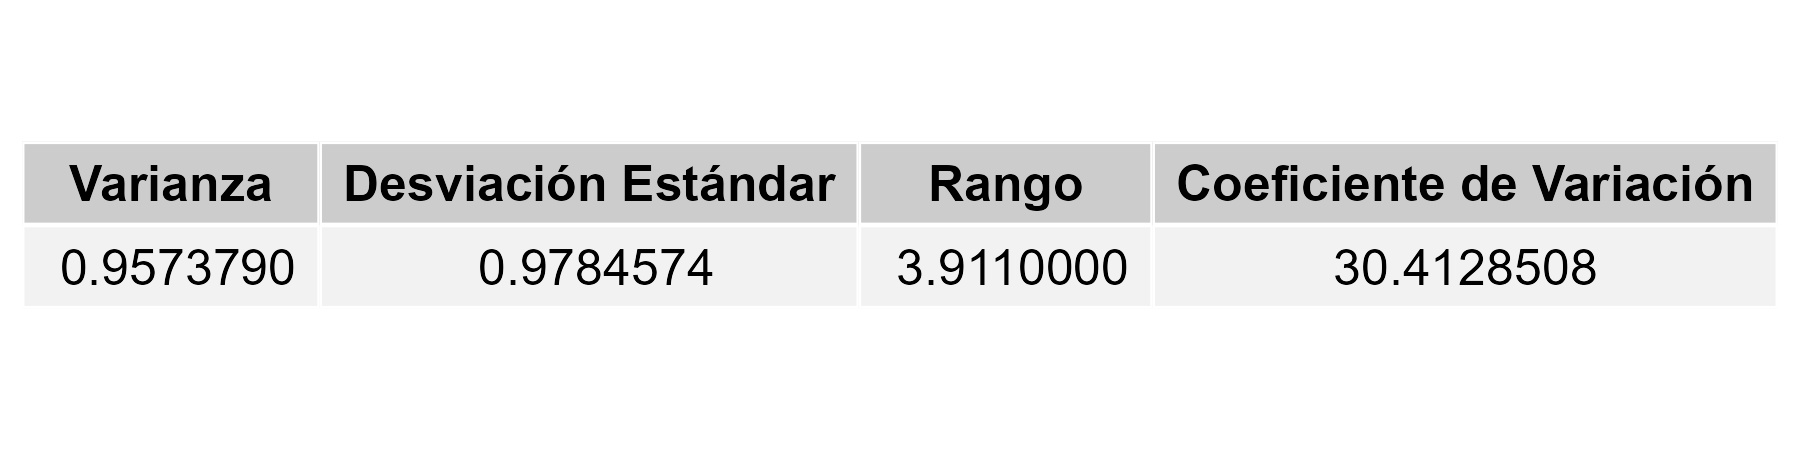
\includegraphics[width=0.8\textwidth]{MTC/wt_dispersion.png}
              \caption{Medidas de dispersión para la variable \texttt{wt}.}
              \label{fig:wt_dispersion}
          \end{figure}

    \item \textbf{qsec (1/4 Mile Time)}

          \begin{itemize}
              \item \textbf{Descripción:} Tiempo en segundos para recorrer un cuarto de milla.
              \item \textbf{Escala:} Cuantitativa Continua.
              \item \textbf{Significado:} Es una medida del tiempo que tarda el automóvil en recorrer un cuarto de milla, comúnmente usado para medir el rendimiento en aceleración.
          \end{itemize}

          \begin{figure}[H]
              \centering
              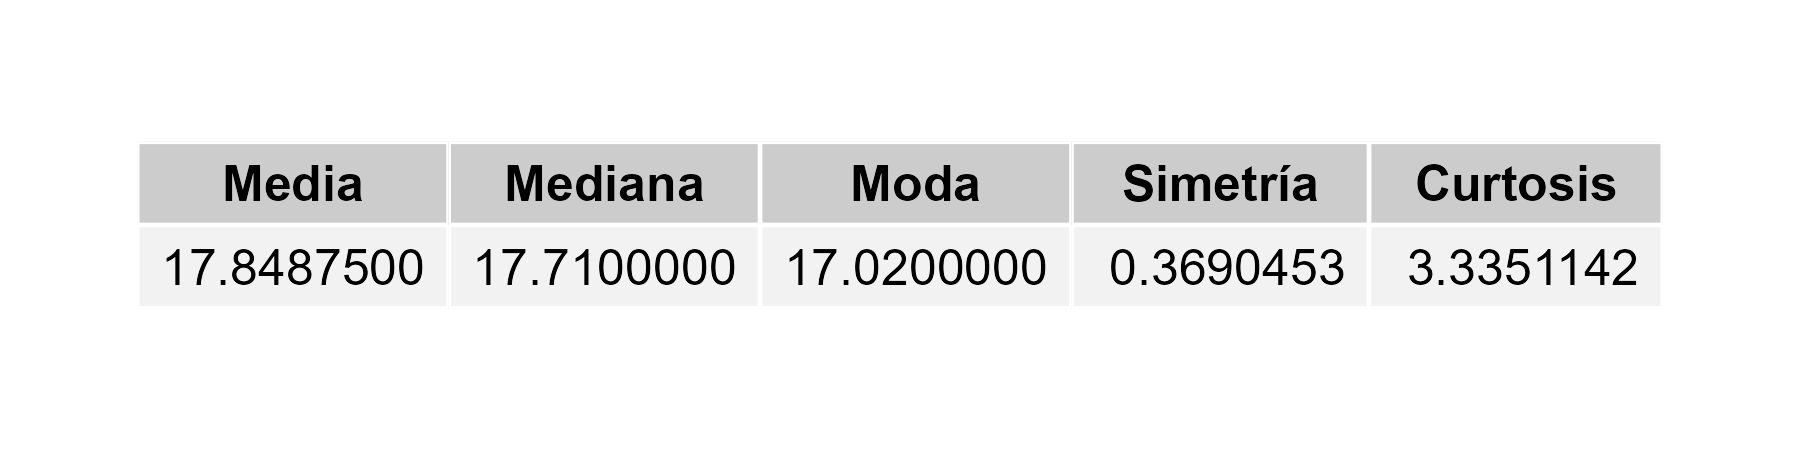
\includegraphics[width=0.8\textwidth]{MTC/qsec_central.png}
              \caption{Medidas de tendencia central para la variable \texttt{qsec}.}
              \label{fig:qsec_central}
          \end{figure}

          \begin{figure}[H]
              \centering
              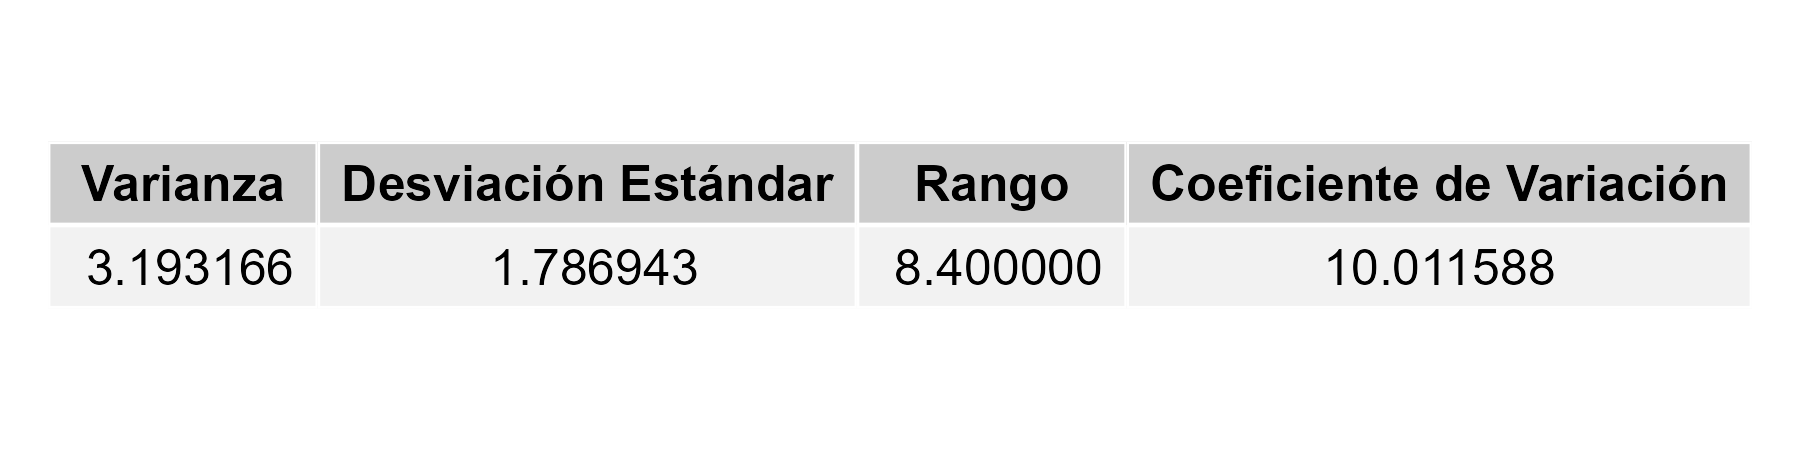
\includegraphics[width=0.8\textwidth]{MTC/qsec_dispersion.png}
              \caption{Medidas de dispersión para la variable \texttt{qsec}.}
              \label{fig:qsec_dispersion}
          \end{figure}

    \item \textbf{vs (Engine Shape)}

          \begin{itemize}
              \item \textbf{Descripción:} Forma del motor (0 = motor en V, 1 = motor en línea).
              \item \textbf{Escala:}  Esta es de cierta manera una variable cualitativa nominal, lo que esta convertida a Cuantitativa Discreta (Binaria).
              \item \textbf{Significado:} Indica el tipo de configuración del motor: si los cilindros están dispuestos en forma de V o en línea.
          \end{itemize}


          \begin{figure}[H]
              \centering
              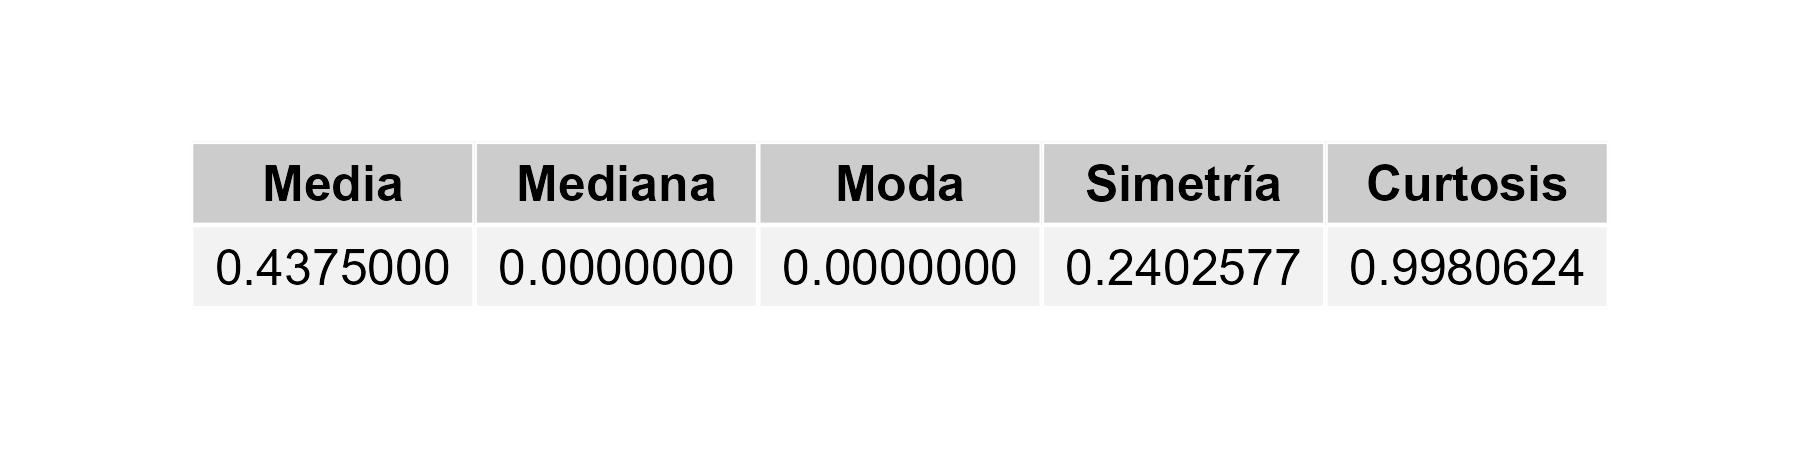
\includegraphics[width=0.8\textwidth]{MTC/vs_central.png}
              \caption{Medidas de tendencia central para la variable \texttt{vs}.}
              \label{fig:vs_central}
          \end{figure}

          \begin{figure}[H]
              \centering
              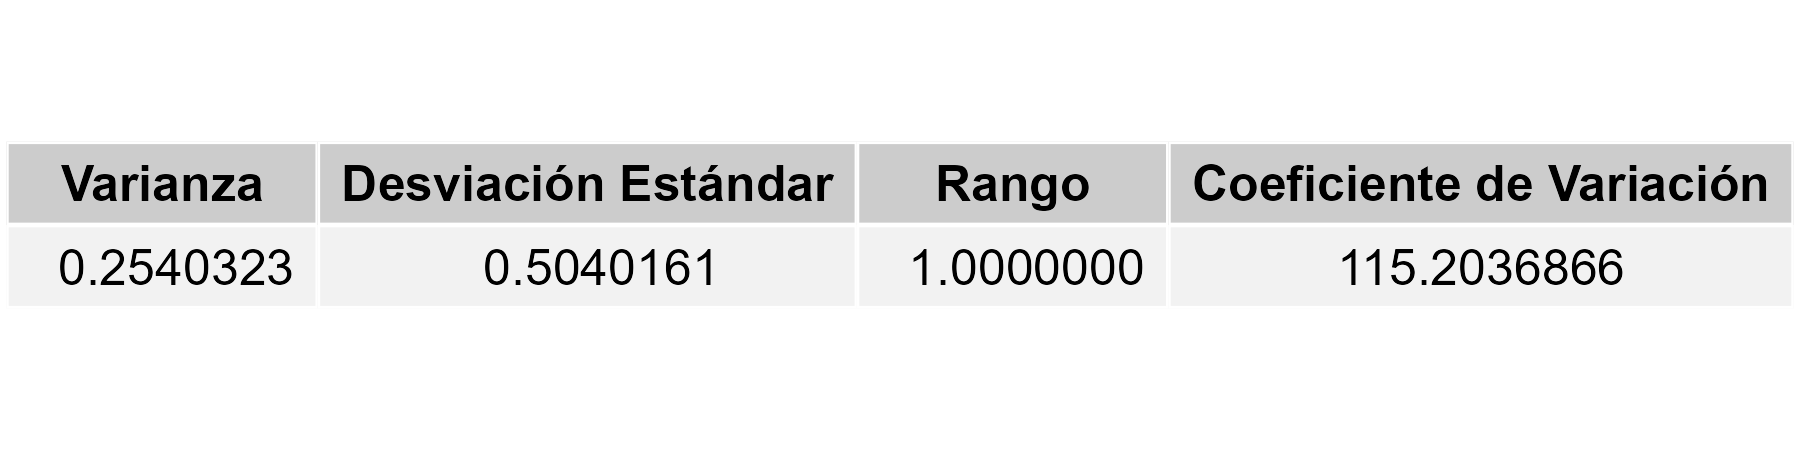
\includegraphics[width=0.8\textwidth]{MTC/vs_dispersion.png}
              \caption{Medidas de dispersión para la variable \texttt{vs}.}
              \label{fig:vs_dispersion}
          \end{figure}

    \item \textbf{am (Transmission)}

          \begin{itemize}
              \item \textbf{Descripción:} Tipo de transmisión (0 = automática, 1 = manual).
              \item \textbf{Escala:} Esta es de cierta manera una variable cualitativa nominal, lo que esta convertida a CUantitativa Discreta (Binaria).
              \item \textbf{Significado:} Indica si el automóvil tiene una transmisión automática o manual.
          \end{itemize}

          \begin{figure}[H]
              \centering
              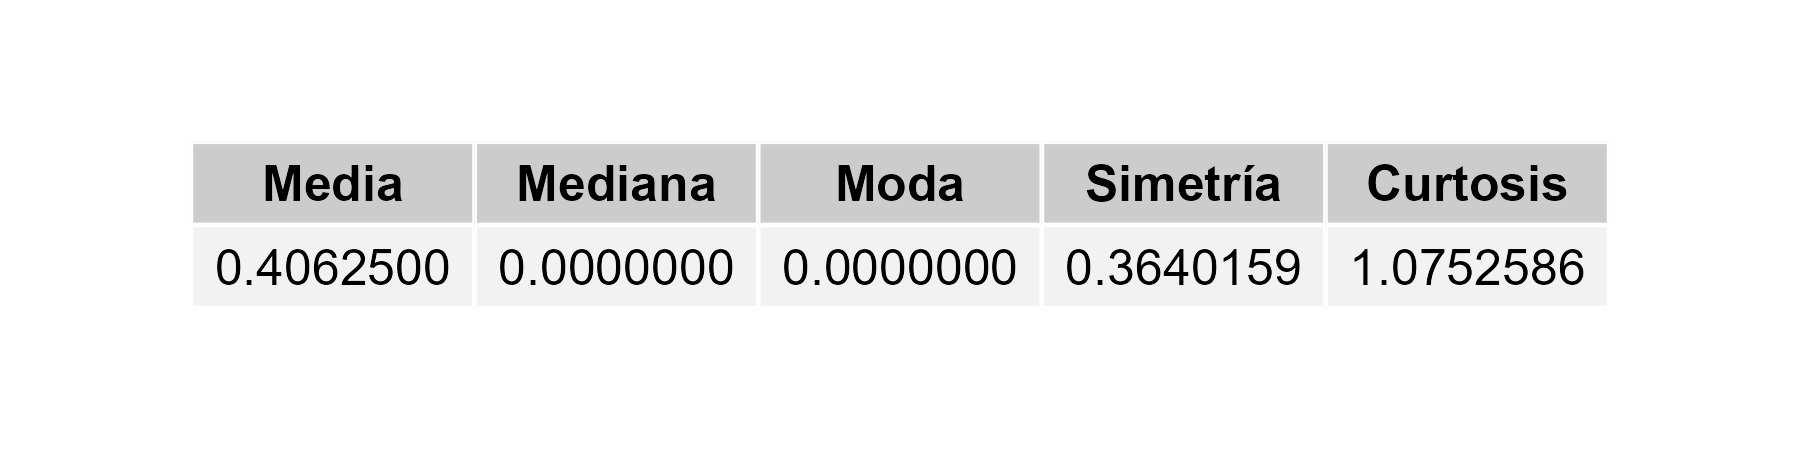
\includegraphics[width=0.8\textwidth]{MTC/am_central.png}
              \caption{Medidas de tendencia central para la variable \texttt{am}.}
              \label{fig:am_central}
          \end{figure}

          \begin{figure}[H]
              \centering
              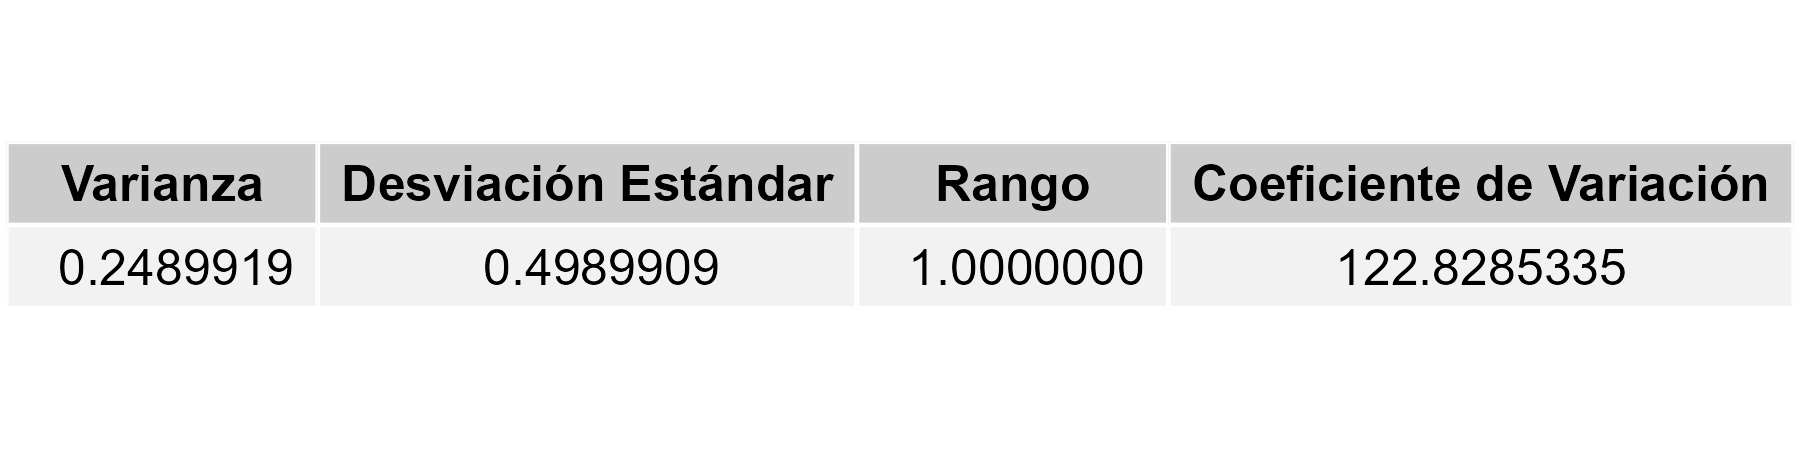
\includegraphics[width=0.8\textwidth]{MTC/am_dispersion.png}
              \caption{Medidas de dispersión para la variable \texttt{am}.}
              \label{fig:am_dispersion}
          \end{figure}

    \item \textbf{gear (Gears)}

          \begin{itemize}
              \item \textbf{Descripción:} Número de velocidades de la caja de cambios.
              \item \textbf{Escala:} Cuantitativa Discreta.
              \item \textbf{Significado:} Indica cuántas marchas tiene la caja de cambios del automóvil.
          \end{itemize}

          \begin{figure}[H]
              \centering
              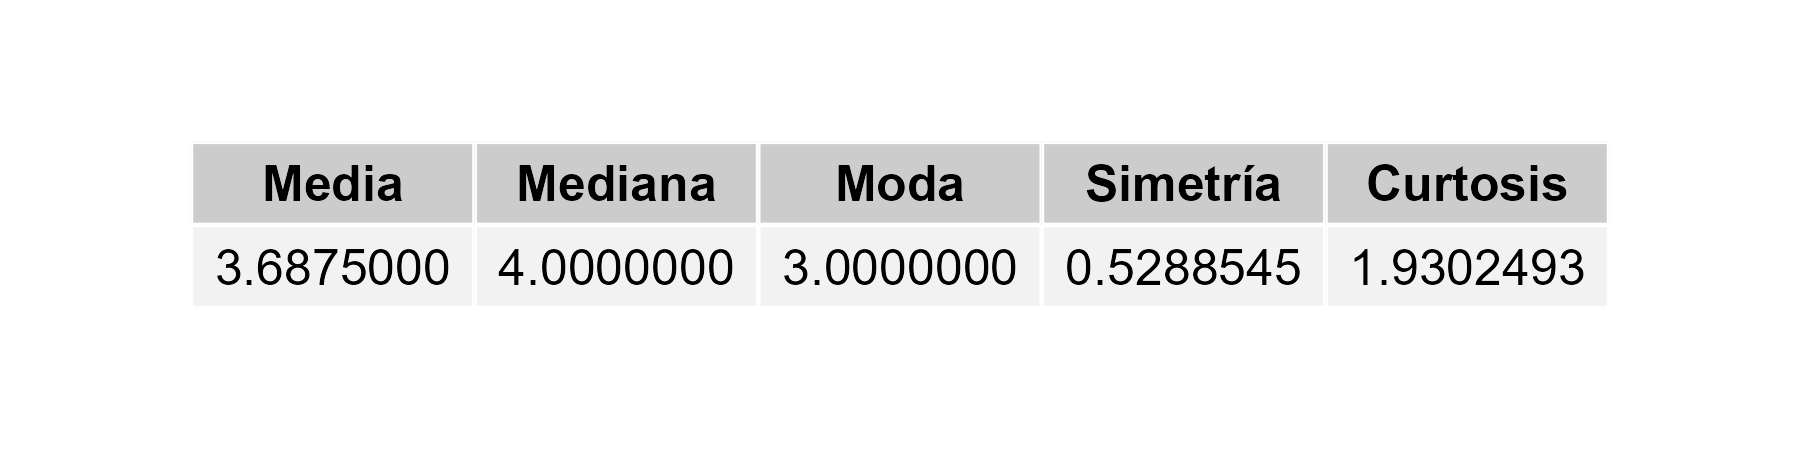
\includegraphics[width=0.8\textwidth]{MTC/gear_central.png}
              \caption{Medidas de tendencia central para la variable \texttt{gear}.}
              \label{fig:gear_central}
          \end{figure}

          \begin{figure}[H]
              \centering
              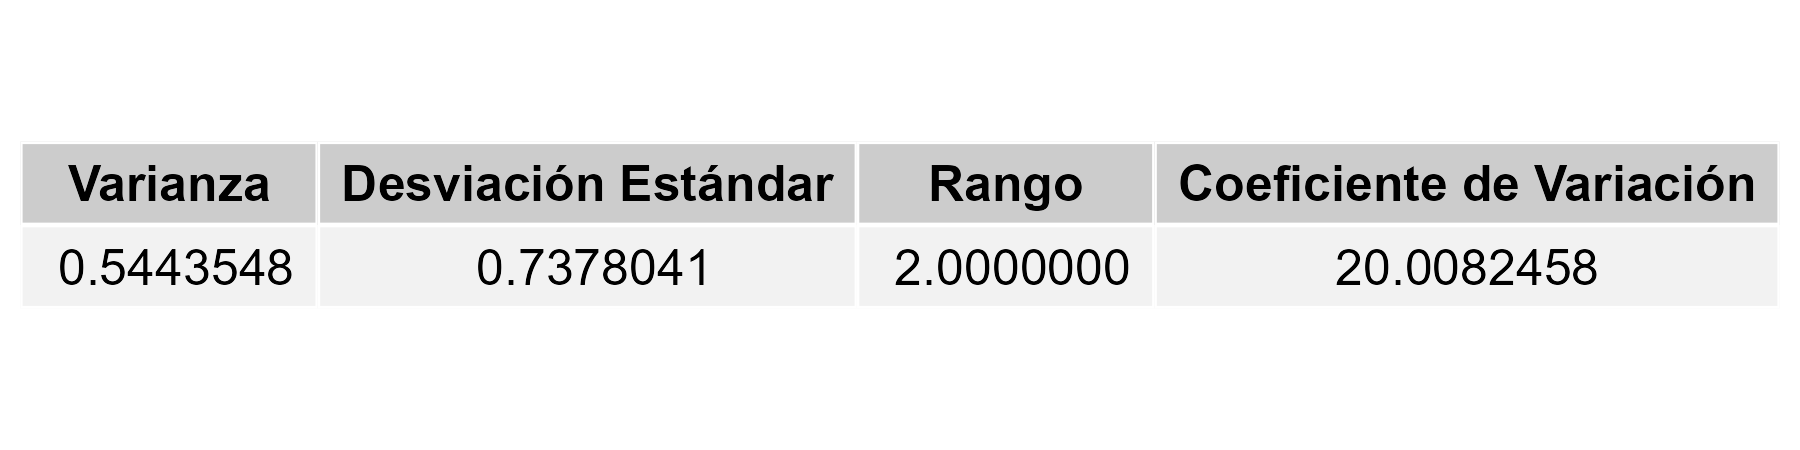
\includegraphics[width=0.8\textwidth]{MTC/gear_dispersion.png}
              \caption{Medidas de dispersión para la variable \texttt{gear}.}
              \label{fig:gear_dispersion}
          \end{figure}

    \item \textbf{carb (Carburetors)}

          \begin{itemize}
              \item \textbf{Descripción:} Número de carburadores.
              \item \textbf{Escala:} Cuantitativa Discreta.
              \item \textbf{Significado:} Indica cuántos carburadores tiene el automóvil, lo que afecta la mezcla de aire y combustible y, por ende, el rendimiento del motor.
          \end{itemize}

          \begin{figure}[H]
              \centering
              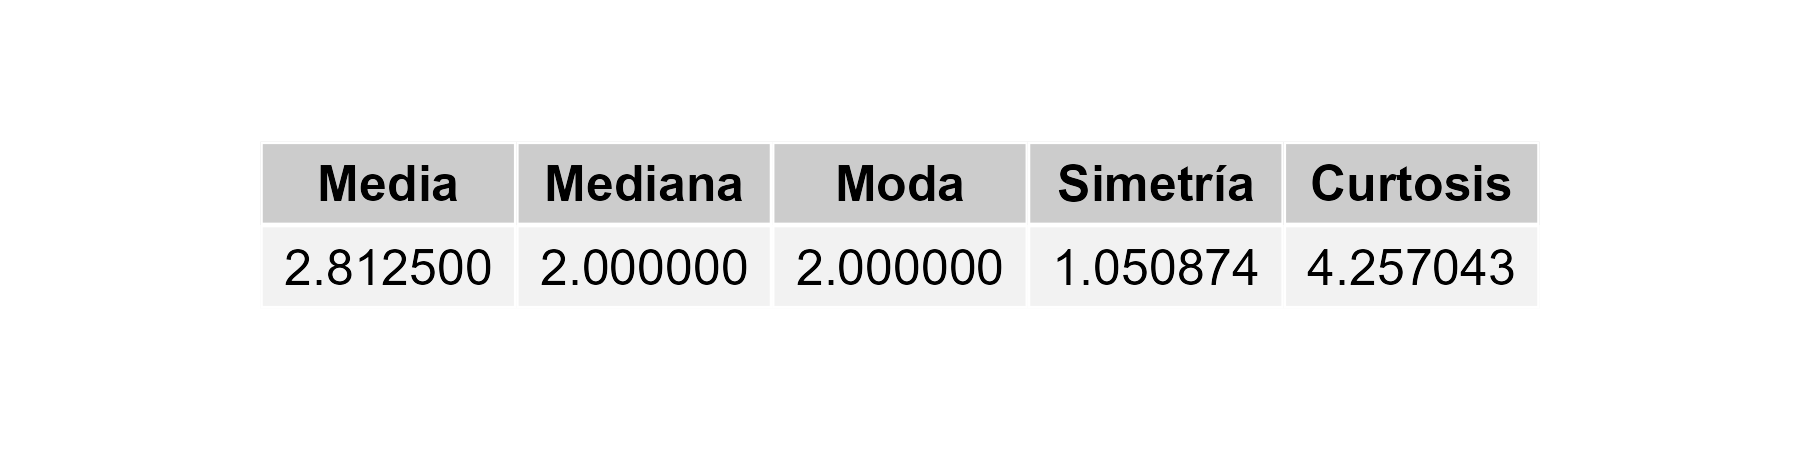
\includegraphics[width=0.8\textwidth]{MTC/carb_central.png}
              \caption{Medidas de tendencia central para la variable \texttt{carb}.}
              \label{fig:carb_central}
          \end{figure}

          \begin{figure}[H]
              \centering
              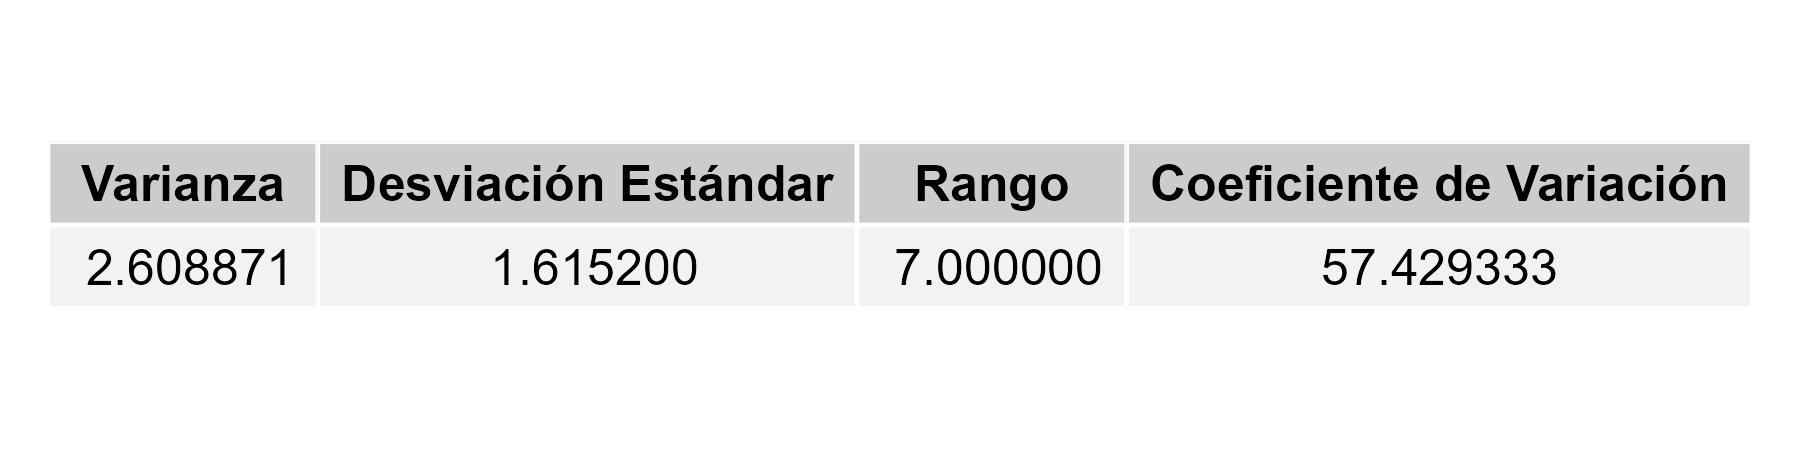
\includegraphics[width=0.8\textwidth]{MTC/carb_dispersion.png}
              \caption{Medidas de dispersión para la variable \texttt{carb}.}
              \label{fig:carb_dispersion}
          \end{figure}

\end{enumerate}

\section{Resultados de la Matriz de Correlación}
A continuación se presentan algunos de los hallazgos clave de la matriz de correlación:

\begin{table}[h]
    \centering
    \begin{tabular}{lccccccccccc}
        \hline
        Variable & mpg   & cyl   & disp  & hp    & drat  & wt    & qsec  & vs    & am    & gear  & carb  \\ \hline
        mpg      & 1.00  & -0.85 & -0.87 & -0.77 & 0.68  & -0.87 & 0.74  & 0.66  & 0.60  & 0.48  & -0.55 \\
        cyl      & -0.85 & 1.00  & 0.90  & 0.78  & -0.50 & 0.87  & -0.59 & -0.81 & -0.52 & 0.36  & 0.55  \\
        disp     & -0.87 & 0.90  & 1.00  & 0.91  & -0.49 & 0.88  & -0.71 & -0.71 & -0.49 & 0.38  & 0.66  \\
        hp       & -0.77 & 0.78  & 0.91  & 1.00  & -0.25 & 0.66  & -0.66 & -0.55 & -0.68 & 0.43  & 0.66  \\
        drat     & 0.68  & -0.50 & -0.49 & -0.25 & 1.00  & -0.39 & 0.11  & 0.13  & 0.79  & 0.29  & -0.09 \\
        wt       & -0.87 & 0.87  & 0.88  & 0.66  & -0.39 & 1.00  & -0.70 & -0.55 & -0.58 & 0.30  & 0.43  \\
        qsec     & 0.74  & -0.59 & -0.71 & -0.66 & 0.11  & -0.70 & 1.00  & 0.74  & 0.59  & -0.17 & -0.55 \\
        vs       & 0.66  & -0.81 & -0.71 & -0.55 & 0.13  & -0.55 & 0.74  & 1.00  & 0.23  & 0.36  & -0.18 \\
        am       & 0.60  & -0.52 & -0.49 & -0.68 & 0.79  & -0.58 & 0.59  & 0.23  & 1.00  & 0.43  & -0.26 \\
        gear     & 0.48  & 0.36  & 0.38  & 0.43  & 0.29  & 0.30  & -0.17 & 0.36  & 0.43  & 1.00  & -0.12 \\
        carb     & -0.55 & 0.55  & 0.66  & 0.66  & -0.09 & 0.43  & -0.55 & -0.18 & -0.26 & -0.12 & 1.00  \\ \hline
    \end{tabular}
    \caption{Matriz de Correlación de las Variables del Dataset mtcars}
    \label{tab:correlation_matrix}
\end{table}


\section{Resumen de Hallazgos}
\begin{itemize}
    \item \textbf{Correlaciones Fuertes}:
          \begin{itemize}
              \item \texttt{mpg} y \texttt{wt}: Correlación negativa fuerte (-0.87), indicando que a mayor peso del automóvil, menor es el rendimiento de combustible.
              \item \texttt{mpg} y \texttt{cyl}: Correlación negativa fuerte (-0.85), sugiriendo que los automóviles con más cilindros tienden a tener un menor rendimiento de combustible.
              \item \texttt{hp} y \texttt{disp}: Correlación positiva fuerte (0.91), indicando que a mayor desplazamiento del motor, mayor es la potencia en caballos de fuerza.
          \end{itemize}
          Lo que tambien es visible en los siguientes graficos de dispersion que relacionan ambas variables

          \begin{figure}[H]
              \centering
              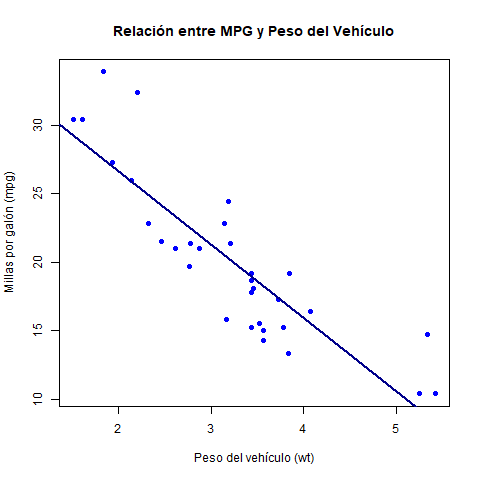
\includegraphics[width=0.5\textwidth]{mpg_vs_wt.png}
              \label{fig:mpg_vs_wt}
              \vspace{0.5cm} % Espacio entre las imágenes
          \end{figure}

          \begin{figure}[H]
              \centering
              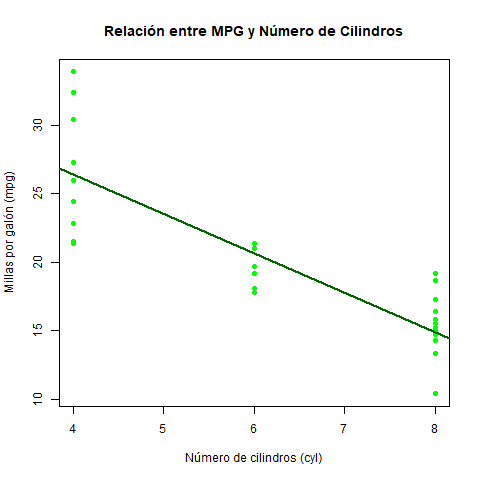
\includegraphics[width=0.5\textwidth]{mpg_vs_cyl.png}
              \label{fig:mpg_vs_cyl}
              \vspace{0.5cm} % Espacio entre las imágenes
          \end{figure}

          \begin{figure}[H]
              \centering
              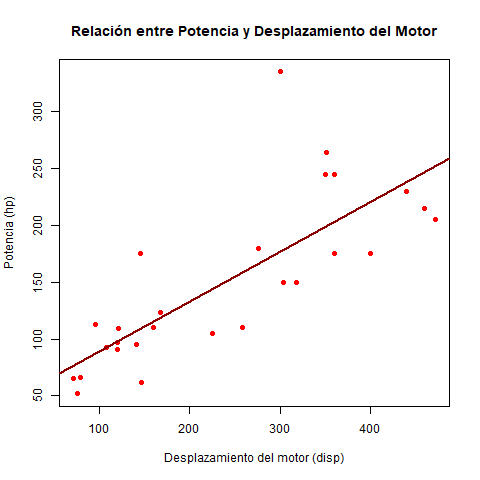
\includegraphics[width=0.5\textwidth]{hp_vs_disp.png}
              \label{fig:hp_vs_disp}
              \vspace{0.5cm} % Espacio entre las imágenes
          \end{figure}

    \item \textbf{Correlaciones Moderadas}:
          \begin{itemize}
              \item \texttt{mpg} y \texttt{drat}: Correlación positiva moderada (0.68), sugiriendo que una mayor relación de transmisión puede estar asociada con un mejor rendimiento de combustible.
              \item \texttt{am} y \texttt{mpg}: Correlación positiva moderada (0.60) entre el tipo de transmisión (manual) y el rendimiento de combustible.
          \end{itemize}

    \item \textbf{Correlaciones Débiles}:
          \begin{itemize}
              \item \texttt{gear} y \texttt{mpg}: Correlación moderada (0.48), indicando que el número de marchas tiene un efecto, pero no tan fuerte como otras variables.La correlación moderada sugiere que el número de marchas puede influir en el rendimiento de combustible, pero no es el único factor. Es decir, un automóvil con más marchas podría tener un mejor rendimiento de combustible, pero hay otras variables (como el peso del automóvil, el tipo de motor, etc.) que también juegan un papel importante.
              \item \texttt{drat} y \texttt{carb}: Correlación débil (-0.09), sugiriendo que no hay una relación significativa entre la relación de transmisión y el número de carburadores.
          \end{itemize}
\end{itemize}

\section{Conclusiones}
El análisis de la matriz de correlación del conjunto de datos \texttt{mtcars} revela varias relaciones significativas entre las variables. Las correlaciones negativas entre el peso y el rendimiento de combustible, así como entre el número de cilindros y el rendimiento de combustible, son particularmente notables. Esto sugiere que los automóviles más pesados y aquellos con más cilindros tienden a ser menos eficientes en términos de consumo de combustible. Por otro lado, las correlaciones positivas entre el desplazamiento y la potencia sugieren que los motores más grandes tienden a ser más potentes.

Estos hallazgos son útiles para comprender cómo las características de los automóviles se relacionan entre sí y pueden guiar decisiones sobre el diseño y la selección de vehículos en función de su rendimiento y eficiencia.
\section{Inserción de Imagen}
A continuación se muestra una imagen:

\begin{figure}[h] % 'h' indica que la imagen debe aparecer aquí
    \centering % Centra la imagen
    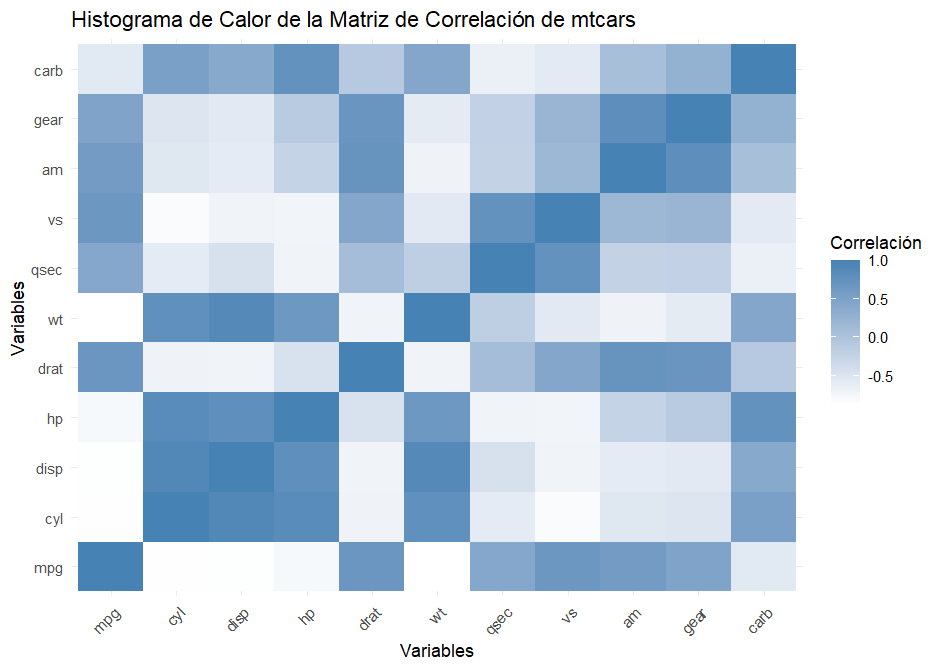
\includegraphics[width=0.8\textwidth]{imagen.png}
    \caption{Grafico de Calor , Correlaciones } % Título de la figura
    \label{fig:mi_imagen} % Etiqueta para referencias cruzadas
\end{figure}
\section{Analisis de la distribucion de Chi-Cuadrado}

\section{Descripción del Gráfico}

\subsection{Ejes del Gráfico}
\begin{itemize}
    \item \textbf{Eje X (Tipo de Transmisión)}: Este eje representa el tipo de transmisión de los automóviles, donde:
          \begin{itemize}
              \item 0 representa transmisión automática.
              \item 1 representa transmisión manual.
          \end{itemize}
    \item \textbf{Eje Y (Frecuencia)}: Este eje muestra la frecuencia observada de automóviles para cada combinación de tipo de transmisión y tipo de motor.
\end{itemize}

\subsection{Barras}
\begin{itemize}
    \item Cada barra representa la frecuencia de automóviles que tienen una combinación específica de tipo de transmisión y tipo de motor.
    \item Las barras están agrupadas por el tipo de transmisión (automática y manual) y se diferencian por color según el tipo de motor:
          \begin{itemize}
              \item 0 representa un motor en línea.
              \item 1 representa un motor en V.
          \end{itemize}
\end{itemize}

\subsection{Colores}
Los colores de las barras indican el tipo de motor. Esto permite una comparación visual rápida entre las frecuencias de los diferentes tipos de motores para cada tipo de transmisión.

\section{Análisis del Gráfico}

\subsection{Comparación de Frecuencias}
Al observar las alturas de las barras, puedes comparar cuántos automóviles tienen transmisión automática frente a manual para cada tipo de motor. Por ejemplo, si la barra para transmisión manual y motor en línea es más alta que la de transmisión automática y motor en línea, esto indica que hay más automóviles con transmisión manual que automática en esa categoría.

\subsection{Tendencias Observadas}
Puedes identificar tendencias en la distribución de los tipos de transmisión y motor. Por ejemplo:
\begin{itemize}
    \item Si hay más automóviles con transmisión manual que automática para ambos tipos de motor, esto podría sugerir una preferencia por la transmisión manual en el conjunto de datos.
    \item Si la frecuencia de motores en línea es mayor en un tipo de transmisión en comparación con el otro, esto puede indicar una relación entre el tipo de transmisión y el tipo de motor.
\end{itemize}

\subsection{Relación entre Variables}
El gráfico permite evaluar visualmente si existe una relación entre el tipo de transmisión y el tipo de motor. Si las frecuencias son muy diferentes entre las combinaciones, esto sugiere que podría haber una asociación significativa entre estas variables. Si las frecuencias son similares, podría indicar que el tipo de transmisión no está relacionado con el tipo de motor.

\section{Conclusion Distribucion Chi-Cuadrado}
\begin{itemize}
    \item El gráfico de barras es una herramienta poderosa para visualizar la relación entre dos variables categóricas.
    \item Permite identificar patrones, tendencias y posibles asociaciones entre las variables.
    \item Junto con los resultados de la prueba chi-cuadrado, este gráfico proporciona una comprensión más profunda de cómo se distribuyen las frecuencias de los automóviles según su tipo de transmisión y motor.
\end{itemize}
\begin{figure}[H] % 'h' indica que la imagen debe aparecer aquí
    \centering % Centra la imagen
    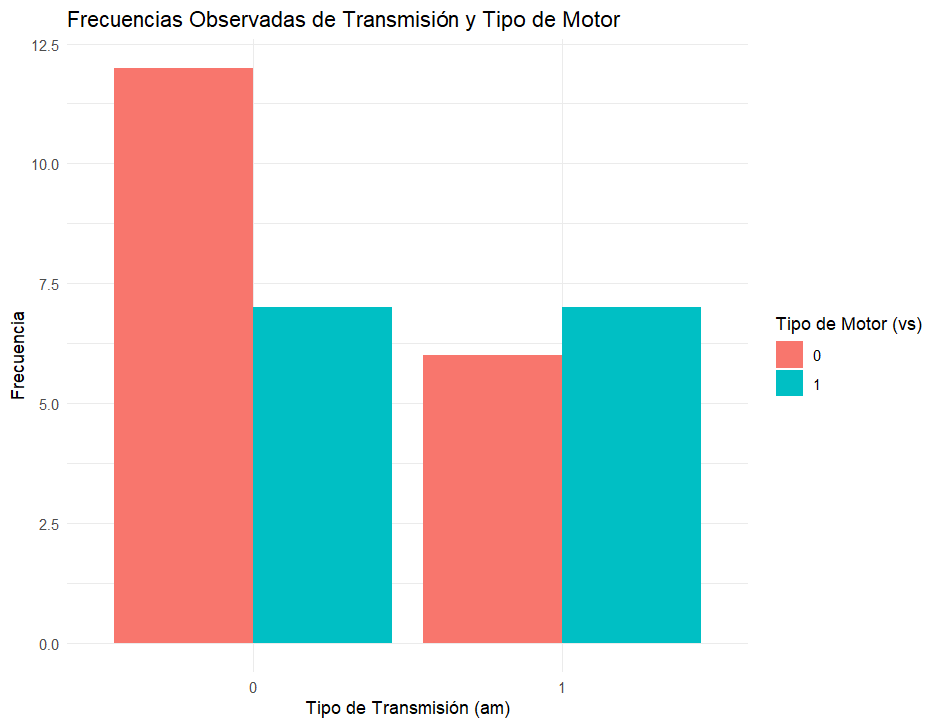
\includegraphics[width=0.8\textwidth]{Imagen2.png}
    \caption{Grafico de Barras, Distribucion Chi-Cuadrado} % Título de la figura
    \label{fig:mi_imagen} % Etiqueta para referencias cruzadas
\end{figure}

\section{Análisis del Histograma de Distribucion Normal\texttt{mpg} }

\subsection{Forma de la Distribución}
El histograma de \texttt{mpg} muestra una distribución que generalmente se asemeja a una campana, lo que sugiere que la mayoría de los automóviles tienen un rendimiento de combustible cercano a la media. La presencia de una forma de campana indica que los datos pueden aproximarse a una distribución normal, aunque es importante verificar esto con pruebas estadísticas adicionales.

\subsection{Frecuencia de Valores}
Las barras del histograma indican la frecuencia de automóviles en diferentes intervalos de \texttt{mpg}. Por ejemplo, si la barra correspondiente al intervalo de 15-20 \texttt{mpg} es más alta, esto significa que hay más automóviles en ese rango de eficiencia de combustible. Además, se puede observar cuántos automóviles tienen un \texttt{mpg} bajo (por ejemplo, menos de 15) en comparación con aquellos que tienen un \texttt{mpg} alto (por ejemplo, más de 30).

\subsection{Media y Desviación Estándar}
La media de \texttt{mpg} puede ser visualmente estimada en el histograma. Si la mayoría de las barras se agrupan alrededor de un valor central, esto indica que la media se encuentra en ese rango. Por otro lado, la desviación estándar se puede inferir observando la dispersión de las barras: un rango más estrecho de barras indica una menor variabilidad, mientras que un rango más amplio sugiere mayor variabilidad en el rendimiento de combustible.Una desviación estándar de 6.03 para datos que varían entre 10 y 33 indica una alta dispersión relativa. Esto puede ser relevante en contextos donde se espera que los datos sean más homogéneos.

\subsection{Identificación de Valores Atípicos}
El histograma puede ayudar a identificar valores atípicos (outliers). Si hay barras que se extienden significativamente más allá de la mayoría de las otras, esto podría indicar la presencia de automóviles con un rendimiento de combustible inusualmente bajo o alto. Por ejemplo, si hay un automóvil que tiene un \texttt{mpg} muy bajo (por debajo de 10), esto podría ser un valor atípico que merece más investigación.

\subsection{Comparación de Rangos de \texttt{mpg}}
Al observar el histograma, se puede comparar la frecuencia de automóviles en diferentes rangos de \texttt{mpg}. Esto ayuda a identificar qué rangos son más comunes y cuáles son menos frecuentes. Por ejemplo, si notas que hay pocos automóviles con un \texttt{mpg} superior a 30, esto sugiere que los automóviles más eficientes en combustible son menos comunes en el conjunto de datos.

\subsection{Tendencias Generales}
A través del histograma, se pueden identificar tendencias generales en el rendimiento de combustible de los automóviles en el conjunto de datos. Esto puede ser útil para entender el mercado automotriz o para realizar análisis de eficiencia energética. Si la mayoría de los automóviles tienen un \texttt{mpg} en el rango de 20-25, esto podría indicar que los vehículos en este conjunto de datos son relativamente eficientes en comparación con los estándares de consumo de combustible.

\subsection{Conclusión de la Distribucion Normal}
El análisis del histograma de \texttt{mpg} proporciona información valiosa sobre la distribución del rendimiento de combustible en el conjunto de datos \texttt{mtcars}. Permite visualizar la forma de la distribución, identificar frecuencias, evaluar la media y la variabilidad, detectar valores atípicos y comprender las tendencias generales en el rendimiento de los automóviles. Este análisis es fundamental para realizar inferencias estadísticas y tomar decisiones informadas sobre el rendimiento de combustible de los vehículos.
\begin{figure}[h] % 'h' indica que la imagen debe aparecer aquí
    \centering % Centra la imagen
    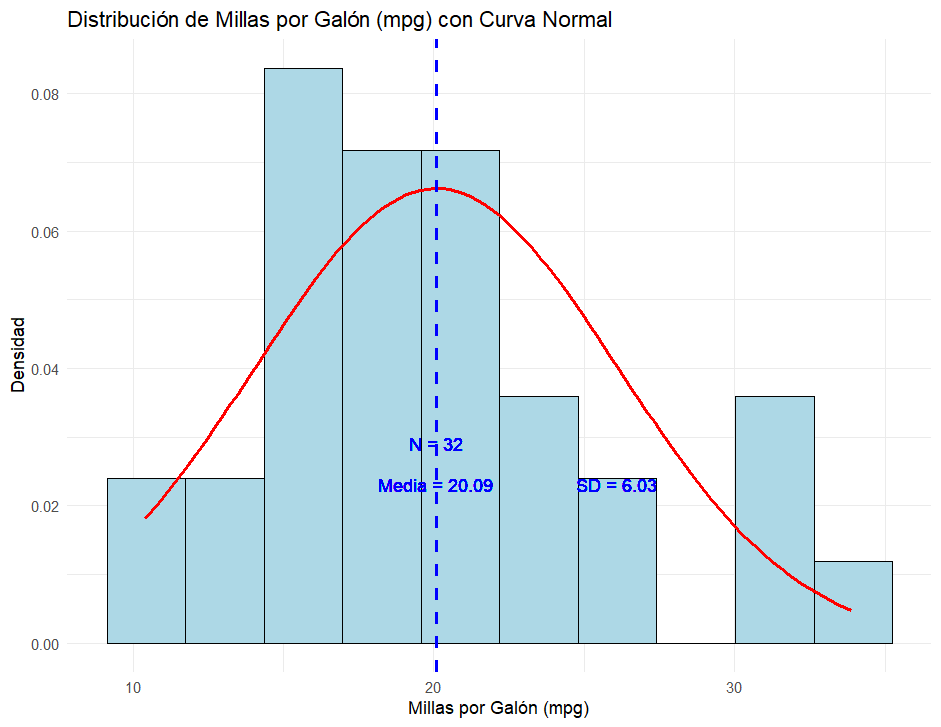
\includegraphics[width=0.8\textwidth]{Image3.png}
    \caption{Distribucion Normal} % Título de la figura
    \label{fig:mi_imagen} % Etiqueta para referencias cruzadas
\end{figure}

\end{document}
